\documentclass[11pt,a4paper]{article}

\usepackage[utf8]{inputenc}
\usepackage[T1]{fontenc}
\usepackage{lmodern}
\usepackage[french]{babel}
\usepackage[margin=2.1cm]{geometry}
\usepackage{microtype}
\usepackage{amsmath,amssymb}
\usepackage{booktabs}
\usepackage{array}
\usepackage[table]{xcolor}
\usepackage{graphicx}
\usepackage{caption}
\usepackage[most]{tcolorbox}

\definecolor{navy}{HTML}{1F3864}
\definecolor{bluemid}{HTML}{2E5496}
\definecolor{lightblue}{HTML}{D6E0F0}

\captionsetup{font=small,labelfont={bf,color=navy},labelsep=period}
\graphicspath{{../figures/}}

\newtcolorbox{cle}[1][]{colback=lightblue!40,colframe=navy,boxrule=0.6pt,
  arc=2pt,left=8pt,right=8pt,top=6pt,bottom=6pt,#1}

\title{\vspace{-1.2cm}\color{navy}\bfseries Le seuil de déclenchement de P4\\[2pt]
  \large La marge, et l'accumulation bornée par la dépendance de queue}
\author{Kélian Kaddouri}
\date{27 juillet 2026}

\begin{document}
\maketitle
\vspace{-0.9cm}

\begin{cle}
\textbf{Deux questions à ne pas confondre.} \emph{Quand} un pilier bascule-t-il (la marge)~?
et \emph{combien} de piliers basculent ensemble (l'accumulation, MOVEit)~? La loi normale
convient à la première et pas à la seconde. Cette note traite le déclenchement dans le modèle
\textbf{par pilier} (une entité, cinq piliers), et répond à la remarque \og{}une loi normale
pour le franchissement~?\fg{}.
\end{cle}

\medskip
\noindent\textbf{(1) La marge.} Le déclenchement est un franchissement, $X_j \ge K_j$ avec
$K_j = F^{-1}(1-p_j)$. La loi $F$ de la latente y est une simple \textbf{normalisation}~:
$K_j = F^{-1}(1-p_j)$ reproduit la probabilité marginale $p_j$ quelle que soit $F$. Prendre $F$
normale ne coûte rien ici, et surtout ne réintroduit \emph{pas} de queue fine dans le capital~:
la queue lourde vit dans la \textbf{sévérité} (GPD, $\xi\simeq 0{,}60$), objet séparé du
déclenchement (scripts 02/04). Pour $P_4$, $p_4=0{,}151$ donne $K_4=1{,}03$.

\medskip
\noindent\textbf{(2) La dépendance.} L'accumulation, elle, dépend de la \textbf{copule}, pas de
la marge. Une copule \textbf{gaussienne} a une dépendance de queue supérieure \textbf{nulle}
($\lambda_U=0$)~: elle sous-estime le basculement simultané de plusieurs piliers, exactement le
phénomène MOVEit. Elle contredit d'ailleurs la copule retenue partout ailleurs dans le mémoire~:
une \textbf{Gumbel} ($\theta=1{,}8$, config), choisie pour sa dépendance de queue supérieure
($\lambda_U = 2-2^{1/\theta}=0{,}53$).

\medskip
\begin{center}
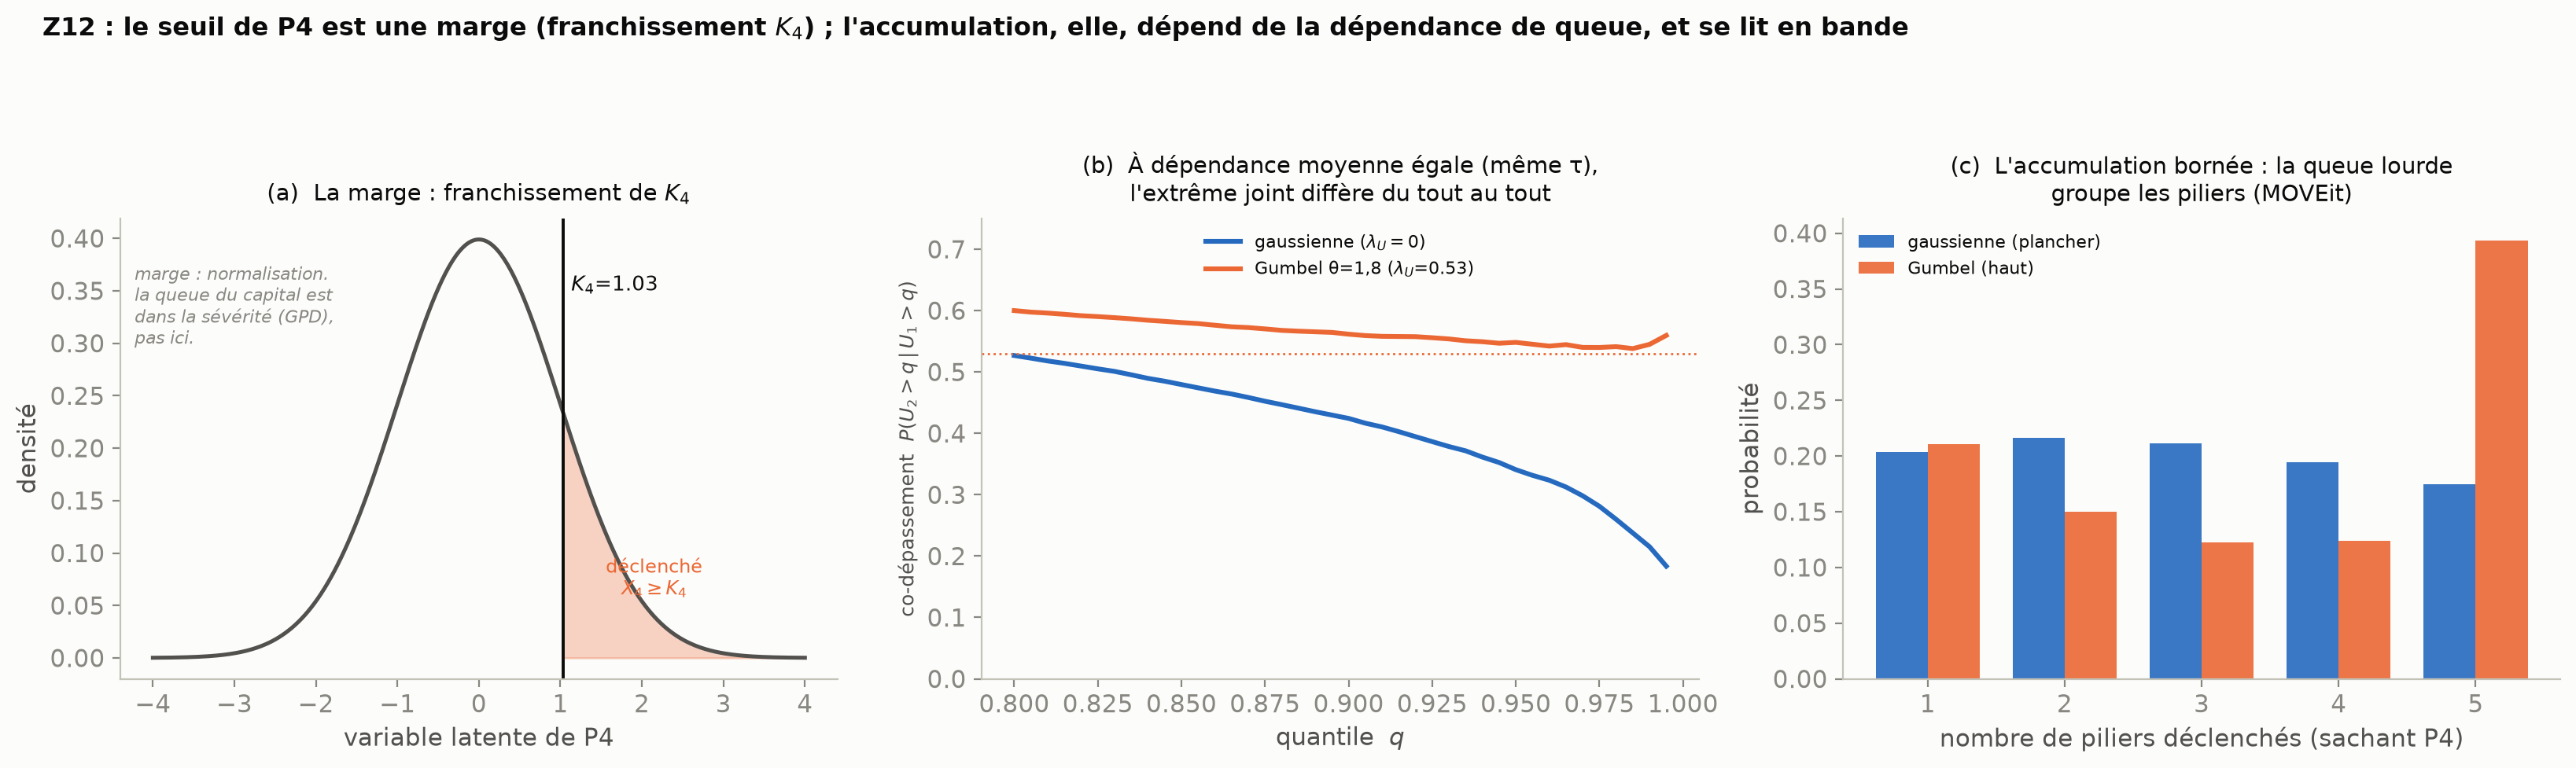
\includegraphics[width=\linewidth]{Z12_seuil_declenchement_p4.png}
\captionof{figure}{\textbf{(a)} la marge~: franchissement de $K_4$, où la normale n'est qu'une
normalisation (la queue du capital est dans la sévérité). \textbf{(b)} à dépendance moyenne
\emph{égale} (même $\tau$ de Kendall), le co-dépassement $P(U_2>q\,|\,U_1>q)$ s'effondre vers
$0$ pour la gaussienne mais plafonne à $0{,}53$ pour la Gumbel~: l'extrême joint diffère du
tout au tout. \textbf{(c)} l'accumulation, lue par pilier~: la Gumbel concentre la masse sur
\emph{les cinq piliers ensemble}, la gaussienne l'étale.}
\end{center}

\begin{cle}
\textbf{Borner l'accumulation, dans l'esprit du mémoire.} On ne tranche pas la copule~: on lit
l'accumulation en \textbf{bande}, à dépendance moyenne égale (même $\tau=0{,}444$), entre le
\textbf{plancher gaussien} ($\lambda_U=0$) et le \textbf{haut de Gumbel} ($\lambda_U=0{,}53$).
La \textbf{marge est invariante} d'une copule à l'autre (chaque pilier bascule seul avec la même
fréquence $p_4=0{,}151$)~: la copule ne change pas \emph{combien} un pilier bascule, mais
\emph{s'ils basculent ensemble}. Les deux copules s'accordent sur le co-déclenchement modéré,
mais divergent sur le \textbf{co-extrême}~: la probabilité que \textbf{les cinq piliers}
tombent avec P4 passe de $0{,}17$ (gaussien) à $0{,}39$ (Gumbel), un facteur $2{,}3$. C'est là
que $\lambda_U$ mord, et c'est le scénario MOVEit.
\end{cle}

\begin{cle}[colback=orange!8,colframe=orange!70!black]
\textbf{Statut et périmètre.} Ce qui est identifié (la marge $p_4$) est posé~; ce qui ne l'est
pas (la dépendance de queue) est lu en bande, jamais en point, même discipline que $W$ et
$\xi$. Le co-déclenchement $\varphi_{cs}=P(\text{un autre pilier}\mid P_4)$ tient dans
$[0{,}48\,;\,0{,}58]$, sous la borne $\gamma=0{,}68$ du script~38, qui reçoit ainsi son origine
structurelle. \textbf{Périmètre}~: tout est par pilier, à une entité (un nombre de piliers, pas
une fraction de portefeuille)~; la vue inter-clients (masse d'entités victimes d'un même
prestataire, vraie maille de MOVEit) serait une loi de Vasicek en dimension \emph{entité},
\textbf{hors} du SCR par entité modélisé ici.
\end{cle}

\smallskip
\noindent\footnotesize\textcolor{navy}{\textbf{Source.}} Script
\texttt{6\_contagion/42\_seuil\_declenchement\_p4.py}, figure
\texttt{Z12\_seuil\_declenchement\_p4.png}. Prolonge 02/04 (seuil $K_j$) et 38 (accumulation P4).
Copule de Gumbel échantillonnée par frailty de Marshall-Olkin (stable positive de Kanter),
$\tau$ empirique vérifié à $0{,}445$.

\end{document}
